\chapter{IMPLEMENTATION} 
\label{sec.implementation}
Based on the design introduced in \S{\ref{sec.design}}, we implement \sysname, a secure network testbed for home wireless routers. It is important to acknowledge that the \sysname benefits from the design and implementation experience of Seattle Testbed~\cite{cappos2009seattle}, an open experimental platform for networking and distributed systems research. Over the past six years, the Seattle Testbed has been used in a variety of different experiments across the world. 

In this section, we discuss some implementation details for our design that might be useful for others trying to adopt parts of the components.

\section{Core Components}
\subsection{Sandbox}
\label{sec.sandbox}
The core sandbox - \sandboxname, which builds on Repy (Restricted Python), a Python-based programming language sandbox that minimizes the risk of bugs by providing security isolation and performance isolation. Experimenters using \sysname use this Python-like programming interface to write experiment code. Currently, Repy provides programmers with the ability to read and write files on the disk, send TCP and UDP traffic, and some utility methods to retrieve time etc. In order to run broadband and wireless network experimentation on home wireless routers, \sysname extends and adds the capabilities to access linux kernel API (e.g., \texttt{iw}) and active measurement tools (e.g., \texttt{ping}, \texttt{traceroute}). The programming interface exposed to the repy-scripts has been extended to include methods to list available access points and connected clients, receive network traffic data from \texttt{/proc} file system and do common active measurements (Ping and Traceroute). To avoid resource limitation, we define a non-renewable (i.e., time independent, such as RAM space) and fungible resource (i.e., interchangeable, such as disk space, CPU)~\cite{li2015fence} to control the resource of reading \texttt{/proc} file system. 

Another important feature of \sandboxname is it allows us to define a policy for its programming interface. For example, the sandbox can anonymize the MAC address of available access points and blacklist home user's LAN. The policy enforcement is presented in \S{\ref{sec.policy}}. We focus on the security and performance isolation of \sandboxname in this section.
\begin{itemize}
\item \textbf{Performance isolation: }Each router running \sysname uses an uniform resource control method to allocate a fixed percentage (usually 50\%) of the router's CPU, memory, bandwidth, disk and other resources to one or more sandboxes. To achieve this, Repy uses operating system hooks to monitor the amount of CPU and memory available to an experiment. To restrict other resources such as network bandwidth and disk I/O, Repy checks those calls that access these resources, and preventing or delaying the execution of these calls if they exceed configured quota. When a router running \sysname boots, it reads a text file that lists the resources allocated to the experiment. Each line contains a resource type and quantity. For example, \texttt{resource diskused 100000000} means that 100 million bytes disk memory can be used at most. Due to this isolation, sandbox does not allow an experiment to consume a lot of resources and ensure experiment not affect Internet connectivity.

\item \textbf{Security isolation: }Repy sandbox has a small, self-contained kernel as its trusted computing base (TCB). In order to minimize the risk of bugs, the TCB is small (only include classic Python classes) so that it is less likely to have security risks than other complex kernels. This sandbox also uses \textit{security layers} to push library functionality out of the sandbox kernel, therefore it is helpful to mitigate security risks in libraries. 

\end{itemize}
\subsection{Package Builder}
\label{sec.packagebuilder}
Any experimenter can easily obtain a customized installer for \sysname which provides access to sandboxes in any way. The goal of the package builder is make it easy to port our platform to OpenWrt. Currently we use OpenWrt SDK to build installer. These installers can be given out by an experimenter who does not want use a clearinghouse. In addition, these installers can be bundled with other components to allow the experimenter direct control over safe experimental sandboxes on their end user devices.

\subsection{Node Manager}
\label{sec.nodemanager}
Node manager~\cite{nodemanager} ensures that sandboxes are correctly assigned to experimenters and experimenters can control those sandboxes safely. The Node manager is based on prior work on Seattle Testbed, but is customized to OpenWrt. For example, \sysname runs on a home wireless router as a background process. Starting it at booting time of the router is implemented by an init.d script instead of crontab. Cryptographically signed messages are used to perform authentication of remote experimenters who are identified by their public keys. An experimenter can perform actions on the sandbox such as starting and stopping an experiment, uploading code, and collecting files and data. The node manager includes code to traverse NAT gateways and firewalls so that it is contactable even if the router does not have a public IP address. 

\subsection{Software Updater}
\label{sec.softwareupdater}
Software updater allows \sysname-enabled router to search for and update new release automatically. It runs in the background to check with the package builder if there exists a new update per some random amount of time (30min - 1hour). It then downloads the new installer from package builder and replaces the old installer. Since the resources are limited, we opt for downloading update package to \texttt{/tmp} (usually 64MB or 128MB) directory to avoid messing home wireless router up.   

\subsection{Lookup Service}
\label{sec.lookupservice}
A lookup service allows an experimenter to locate corresponding sandboxes. We currently use centralized advertise servers as a distributed way to store data. This central lookup service, which is a centralized hash table abstraction, is used to decrease lookup redundancy when OpenDHT fails.

\subsection{Experiment Manager}
\label{sec.seash}
An experiment manager provides experimenters with a simple interface for interacting with the resource manager on remote devices. The primary interactive service manager used in \sysname is \textit{seash}~\cite{seash}. It provides an interactive shell to the experimenters, and exchanges cryptographically signed communication with sandboxes to control experiments and upload files. Also, the experiment manager supports contacting routers in networks behind NAT gateways and firewalls to satisfy the reality of today's network.

\section{Sandbox Extensions}
\label{sec.extensions}
Extensions enhance the functionality of the Repy sandbox and allow a wide range of network measurements on a home wireless router. First, we implemented system hooks call \textit{openwrt module} to interact with a variety of wired and wireless network information through a Linux kernel API. Currently, implemented \textit{openwrt module} is supported to learn about configured network interfaces statistics, connected devices, nearby WiFi access points and channel utilization. While \textit{openwrt module} provides read access to valuable data, it can not modify data. Additionally, we also implemented \textit{general modules} to provide two active measurement tools (\texttt{ping}~\cite{pingcode} and \texttt{traceroute}~\cite{traceroutecode}). We choose a pure raw socket method to implement them so that they will be supported across a variety of operating systems. 

\textbf{Protecting command injection.} Command injection is an attack in which arbitrary commands are executed on the host operating system by a vulnerable application. A possible reason of a command injection attack is insufficient input validation. \sysname sanitizes the call arguments, handles onerous output parsing, and returns results to the caller. One example is \texttt{scan} implementation. This function will run a system command \texttt{iw dev interface\_name station dump}. Normally, the output is station statistic information. However, if we add a semicolon and another to the end of this line, the command is executed as well, such as \texttt{;ls} could show all files in current directory. We will check whether an interface name is legal, as any illegal arguments will pose a security risk. \sysname API never allows invocation of arbitrary system calls.

\begin{figure}%[h]
\centering
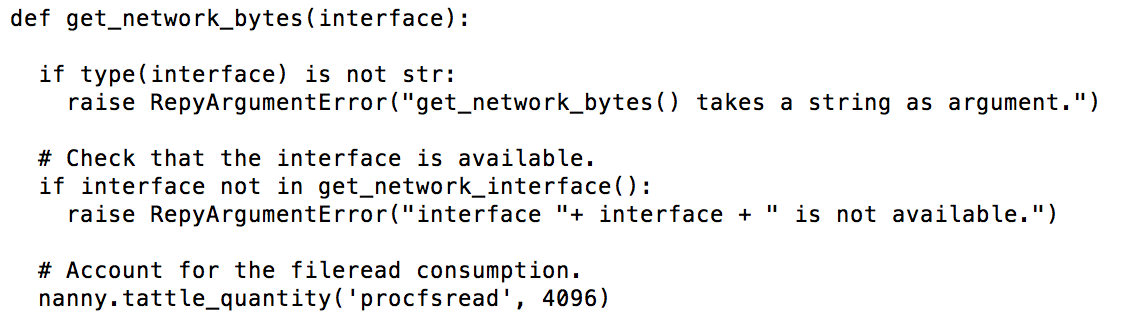
\includegraphics[width=0.8\columnwidth]{figure/nanny.png}
\caption{Additional codes in \sysname sandbox's \texttt{get\_network\_bytes()} call to make sure resource control and command injection protection.}
\label{fig-nanny}
\end{figure}

\textbf{Resource control.} Resource control is an important security mechanism. It provides protection from accidental or deliberate over-usage of resources by APIs that could affect the service level of the end host. Each new function in \sandboxname defines a resource type to record the amount of resource consumed. The specific function made depends on the type of resource being consumed. Figure \ref{fig-nanny} shows some of codes in \texttt{get\_network\_bytes()}. First of all, we check whether the argument is legal and available. The \texttt{tattle\_quantity()} call charges for the consumed fileread. When a \sysname starts, it reads a text file that lists the resources allocated to the platform. Each line contains a resource type and quantity. For example, \texttt{resource procfsread 100000} sets the allowed consumption of reading \texttt{/proc} filesystem to 100 thousand bytes. When experiment codes try to exceed the limit, it will be forcefully stopped.

\section{Sandbox Policies}
\label{sec.policy}
In order for a router owner to participate safely in \sysname, he should have the ability to decide policies on his own. For instance, he should know the amount of resources \sysname will use on his router and the capabilities experiment code can access. We have mentioned the resource control in \S{\ref{sec.sandbox}}. To restrict capabilities, the sandbox in \sysname provides a flexible policy enforcement method that uses Repy's security layer to help a router owner decide policies. The Sandbox can interject code to control the behavior of these calls through a system call interposition technique. Using this technology, a sandbox policy can (1) restrict capability access, such as blocking sending TCP or UDP packet to protect LAN, and (2) reduce precision of returned data from a router, such as returning the number of connected devices rather than detailed information about them.

\subsection{Reducing Data Precision}
Our sandbox may provides potentially inappropriate functions, such as network traffic capture that discloses the home network behavior pattern of the router owner. These kinds of policies are able to change the behavior of a function by disabling the returned value, or the precision of the specified value returned. For instance, a security layer could truncate an access point MAC address to the manufacturer ID.

\begin{figure}%[h]
\centering
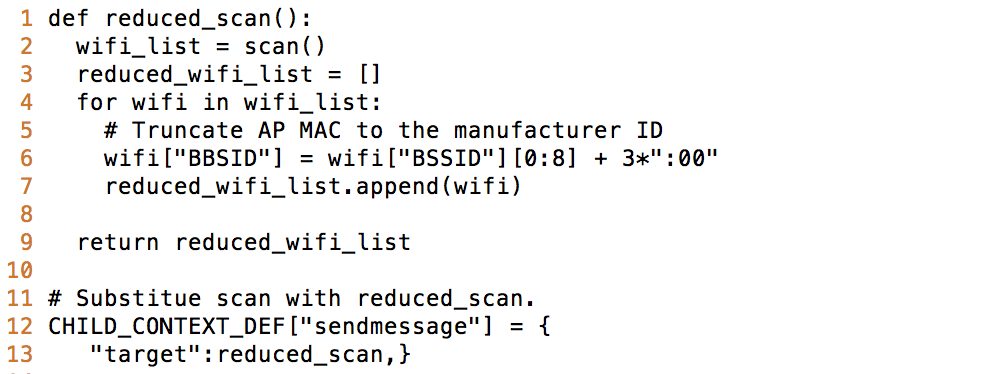
\includegraphics[width=0.8\columnwidth]{figure/example.png}
\caption{Using security layer to define a simple sandbox policy: truncate access point MAC address to the manufacturer ID.}
\label{fig-examplecode1}
\end{figure}

As shown in Figure~\ref{fig-examplecode1}, whenever experiment code calls \texttt{scan()}, the security layer above replaces it with \texttt{reduced\_scan()}. Therefore, security layer is able to ensure the router owner's policy.

\subsection{Restricting Capability Access}
This kind of policy is able to allow experimenters to restrict the code on a home wireless router. For example, the experimenter might want to restrict part of functionalities to satisfy router owner's need. It is also useful to save time in vetting experiment code because most harmful capabilities are restricted. As a result, \sysname is able to maintain containment of experiment code despite bugs in its libraries.

\begin{figure}%[h]
\centering
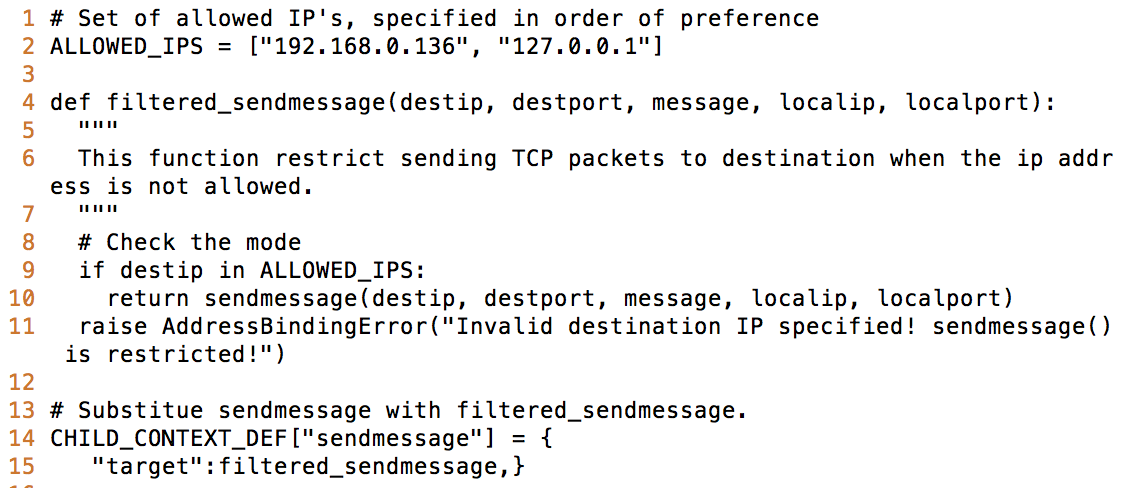
\includegraphics[width=0.8\columnwidth]{figure/example-restrict_data.png}
\caption{Using security layer to define a simple sandbox policy: Restrict \texttt{sendmessage} function when the destination is not allowed IP address.}
\label{fig-examplecode2}
\end{figure}

As shown in Figure~\ref{fig-examplecode2}, whenever experiment code calls \texttt{sendmessage}, the security layer above replaces it with \texttt{filtered\_sendmessage}. In that way, hackers would not have the ability of writing a program which exploits TCP vulnerabilities to connect and gain immediate privileged access to Wi-Fi enabled devices in home networks. 

 